\documentclass[tikz,border=10pt]{standalone}
\usepackage[T1]{fontenc}
\usepackage{tgheros}
\usepackage{sfmath}
\usepackage{amsmath}
\usepackage{tikz}
\usetikzlibrary{arrows.meta,positioning,shapes.geometric,fit,backgrounds,calc}
\usepackage{xcolor}

\renewcommand{\familydefault}{\sfdefault}

% Academic Semantic Palette (Harvard Crimson & ETH Zurich)
\definecolor{ethdarkblue}{HTML}{1F407A}
\definecolor{ethblue}{HTML}{215CAF}
\definecolor{ethpetrol}{HTML}{007A87}
\definecolor{ethbronze}{HTML}{B87333}
\definecolor{harvardcrimson}{HTML}{A51C30}
\definecolor{ethslate}{HTML}{334155}
\definecolor{cardbg}{HTML}{F8FAFC}
\definecolor{cardborder}{HTML}{CBD5E1}
\definecolor{subtlebg}{HTML}{F1F5F9}

\begin{document}
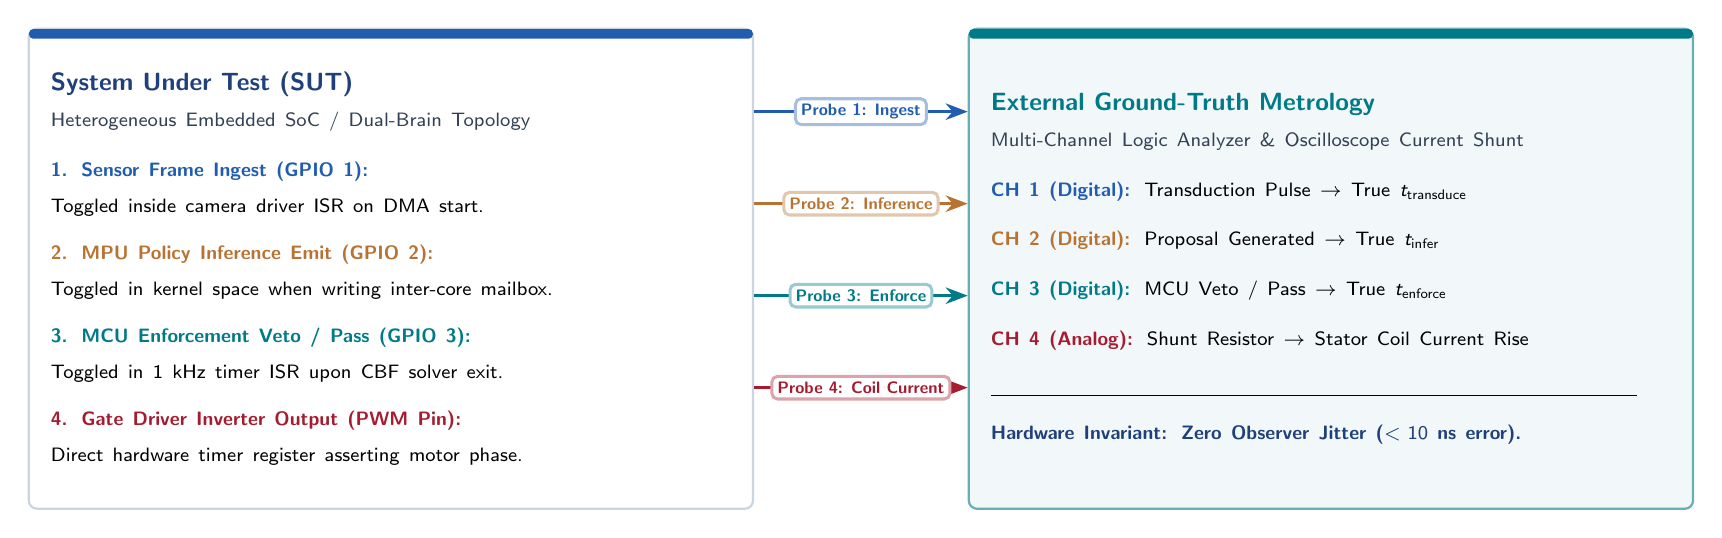
\begin{tikzpicture}[
  font=\sffamily,
  >=Stealth,
  scale=1.0,
  sutbox/.style={
    draw=cardborder,
    fill=white,
    rounded corners=3pt,
    line width=0.8pt,
    text width=3.40in,
    minimum height=2.40in,
    inner sep=8pt,
    align=left,
    anchor=north
  },
  scopebox/.style={
    draw=ethpetrol!60,
    fill=ethpetrol!5,
    rounded corners=3pt,
    line width=0.8pt,
    text width=3.40in,
    minimum height=2.40in,
    inner sep=8pt,
    align=left,
    anchor=north
  }
]

  % ---------------------------------------------------------------------------
  % SUT (System Under Test)
  % ---------------------------------------------------------------------------
  \node[sutbox] (dut) at (0, 0) {
    {\fontsize{9pt}{11.5pt}\selectfont\bfseries\color{ethdarkblue}System Under Test (SUT)}\\[1pt]
    {\fontsize{7.5pt}{9.5pt}\selectfont\color{ethslate}Heterogeneous Embedded SoC / Dual-Brain Topology}\\[6pt]
    
    {\fontsize{7.5pt}{9.5pt}\selectfont\bfseries\color{ethblue}1. Sensor Frame Ingest (GPIO 1):}\\[1pt]
    {\fontsize{7pt}{8.5pt}\selectfont Toggled inside camera driver ISR on DMA start.}\\[5pt]
    
    {\fontsize{7.5pt}{9.5pt}\selectfont\bfseries\color{ethbronze}2. MPU Policy Inference Emit (GPIO 2):}\\[1pt]
    {\fontsize{7pt}{8.5pt}\selectfont Toggled in kernel space when writing inter-core mailbox.}\\[5pt]
    
    {\fontsize{7.5pt}{9.5pt}\selectfont\bfseries\color{ethpetrol}3. MCU Enforcement Veto / Pass (GPIO 3):}\\[1pt]
    {\fontsize{7pt}{8.5pt}\selectfont Toggled in 1 kHz timer ISR upon CBF solver exit.}\\[5pt]
    
    {\fontsize{7.5pt}{9.5pt}\selectfont\bfseries\color{harvardcrimson}4. Gate Driver Inverter Output (PWM Pin):}\\[1pt]
    {\fontsize{7pt}{8.5pt}\selectfont Direct hardware timer register asserting motor phase.}
  };
  % Accent bar
  \fill[ethblue, rounded corners=1.5pt] ($(dut.north west) + (0.5pt, -0.5pt)$) rectangle ($(dut.north east) + (-0.5pt, -4pt)$);

  % ---------------------------------------------------------------------------
  % EXTERNAL TEST EQUIPMENT (Oscilloscope & Logic Analyzer)
  % ---------------------------------------------------------------------------
  \node[scopebox] (scope) at (4.70in, 0) {
    {\fontsize{9pt}{11.5pt}\selectfont\bfseries\color{ethpetrol}External Ground-Truth Metrology}\\[1pt]
    {\fontsize{7.5pt}{9.5pt}\selectfont\color{ethslate}Multi-Channel Logic Analyzer \& Oscilloscope Current Shunt}\\[6pt]
    
    {\fontsize{7.5pt}{9.5pt}\selectfont\bfseries\color{ethblue}CH 1 (Digital):} {\fontsize{7pt}{8.5pt}\selectfont Transduction Pulse $\to$ True $t_{\text{transduce}}$}\\[6pt]
    {\fontsize{7.5pt}{9.5pt}\selectfont\bfseries\color{ethbronze}CH 2 (Digital):} {\fontsize{7pt}{8.5pt}\selectfont Proposal Generated $\to$ True $t_{\text{infer}}$}\\[6pt]
    {\fontsize{7.5pt}{9.5pt}\selectfont\bfseries\color{ethpetrol}CH 3 (Digital):} {\fontsize{7pt}{8.5pt}\selectfont MCU Veto / Pass $\to$ True $t_{\text{enforce}}$}\\[6pt]
    {\fontsize{7.5pt}{9.5pt}\selectfont\bfseries\color{harvardcrimson}CH 4 (Analog):} {\fontsize{7pt}{8.5pt}\selectfont Shunt Resistor $\to$ Stator Coil Current Rise}\\[6pt]
    
    \rule{0.95\linewidth}{0.3pt}\\[4pt]
    {\fontsize{7.5pt}{9.5pt}\selectfont\bfseries\color{ethdarkblue}Hardware Invariant: Zero Observer Jitter ($< 10\text{ ns}$ error).}
  };
  % Accent bar
  \fill[ethpetrol, rounded corners=1.5pt] ($(scope.north west) + (0.5pt, -0.5pt)$) rectangle ($(scope.north east) + (-0.5pt, -4pt)$);

  % ---------------------------------------------------------------------------
  % CONNECTING PROBES
  % ---------------------------------------------------------------------------
  \draw[->, line width=1.1pt, ethblue] ($(dut.north east) + (0, -0.42in)$) -- ($(scope.north west) + (0, -0.42in)$)
    node[midway, font=\fontsize{6.5pt}{8pt}\selectfont\bfseries, fill=white, draw=ethblue!40, rounded corners=2pt, inner sep=2pt, text=ethblue] {Probe 1: Ingest};

  \draw[->, line width=1.1pt, ethbronze] ($(dut.north east) + (0, -0.88in)$) -- ($(scope.north west) + (0, -0.88in)$)
    node[midway, font=\fontsize{6.5pt}{8pt}\selectfont\bfseries, fill=white, draw=ethbronze!40, rounded corners=2pt, inner sep=2pt, text=ethbronze] {Probe 2: Inference};

  \draw[->, line width=1.1pt, ethpetrol] ($(dut.north east) + (0, -1.34in)$) -- ($(scope.north west) + (0, -1.34in)$)
    node[midway, font=\fontsize{6.5pt}{8pt}\selectfont\bfseries, fill=white, draw=ethpetrol!40, rounded corners=2pt, inner sep=2pt, text=ethpetrol] {Probe 3: Enforce};

  \draw[->, line width=1.1pt, harvardcrimson] ($(dut.north east) + (0, -1.80in)$) -- ($(scope.north west) + (0, -1.80in)$)
    node[midway, font=\fontsize{6.5pt}{8pt}\selectfont\bfseries, fill=white, draw=harvardcrimson!40, rounded corners=2pt, inner sep=2pt, text=harvardcrimson] {Probe 4: Coil Current};

\end{tikzpicture}
\end{document}
